% Practice Test 07 — Texas Edition
% Questions: 30 (18 MC + 12 SA)
% Generated by scripts/generate_practice_tests.py

\begin{practiceQuestion}{1-3-q23}{sa}
\begin{questionText}
Two quantities are proportional with $k = 7$. If $y = 56$, what is $x$?
\end{questionText}
\correctAnswer{$x = 8$}
\explanation{$y = kx$ so $56 = 7x$, giving $x = 56 \div 7 = 8$.}
\end{practiceQuestion}

\begin{practiceQuestion}{1-6-q09}{mc}
\begin{questionText}
Which strategy is NOT a proportional reasoning tool?
\end{questionText}
\choiceA{Find the unit rate and multiply}
\choiceB{Set up a proportion and cross-multiply}
\choiceC{Use $y = kx$}
\choiceD{Add a fixed amount to each value}
\correctAnswer{D}
\explanation{Adding a fixed amount is an additive strategy, not proportional. Proportional strategies use multiplication and division.}
\end{practiceQuestion}

\begin{practiceQuestion}{2-1-q29}{gsa}
\begin{questionText}
Look at the $10 \times 10$ grid below. What percent of the grid is \textbf{not} shaded?

\begin{center}
\begin{tikzpicture}[scale=0.35]
  \foreach \x in {0,...,9} {
    \foreach \y in {0,...,9} {
      \draw[gray!50] (\x,\y) rectangle (\x+1,\y+1);
    }
  }
  % Shade 72 squares (rows 0-6 full = 70, plus 2 in row 7)
  \foreach \x in {0,...,9} {
    \foreach \y in {0,...,6} {
      \fill[funOrange!40] (\x,\y) rectangle (\x+1,\y+1);
      \draw[gray!50] (\x,\y) rectangle (\x+1,\y+1);
    }
  }
  \foreach \x in {0,...,1} {
    \fill[funOrange!40] (\x,7) rectangle (\x+1,8);
    \draw[gray!50] (\x,7) rectangle (\x+1,8);
  }
\end{tikzpicture}
\end{center}
\end{questionText}
\correctAnswer{$28\%$}
\explanation{Shaded squares: $7$ full rows of $10 = 70$, plus $2 = 72$. Unshaded: $100 - 72 = 28$. So $28\%$ is not shaded.}
\end{practiceQuestion}

\begin{practiceQuestion}{2-3-q27}{gmc}
\begin{questionText}
The double number line shows an original price and a discounted price. What is the percent decrease?

\begin{center}
\begin{tikzpicture}[scale=0.7]
  % Top: price
  \draw[thick,->] (0,1) -- (10.5,1);
  \node[left,font=\small] at (0,1) {Price};
  \draw[thick] (0,0.85) -- (0,1.15); \node[above,font=\small] at (0,1.15) {$\$0$};
  \draw[thick] (6,0.85) -- (6,1.15); \node[above,font=\small] at (6,1.15) {$\$48$};
  \draw[thick] (10,0.85) -- (10,1.15); \node[above,font=\small] at (10,1.15) {$\$80$};
  % Bottom: percent
  \draw[thick,->] (0,0) -- (10.5,0);
  \node[left,font=\small] at (0,0) {\%};
  \draw[thick] (0,-0.15) -- (0,0.15); \node[below,font=\small] at (0,-0.15) {$0\%$};
  \draw[thick] (6,-0.15) -- (6,0.15); \node[below,font=\small] at (6,-0.15) {?};
  \draw[thick] (10,-0.15) -- (10,0.15); \node[below,font=\small] at (10,-0.15) {$100\%$};
  % Arrow showing decrease
  \draw[thick,->,funRed] (10,1.6) to[bend left=20] node[above,font=\small]{discount} (6,1.6);
\end{tikzpicture}
\end{center}
\end{questionText}
\choiceA{$32\%$}
\choiceB{$40\%$}
\choiceC{$48\%$}
\choiceD{$60\%$}
\correctAnswer{B}
\explanation{The sale price $\$48$ is $\frac{48}{80} = 60\%$ of the original. The percent decrease is $100\% - 60\% = 40\%$.}
\end{practiceQuestion}

\begin{practiceQuestion}{2-6-q19}{sa}
\begin{questionText}
Find the simple interest: $P = \$3{,}500$, $r = 4\%$, $t = 2$ years.
\end{questionText}
\correctAnswer{$\$280$}
\explanation{$I = 3{,}500 \times 0.04 \times 2 = \$280$.}
\end{practiceQuestion}

\begin{practiceQuestion}{2-8-q21}{sa}
\begin{questionText}
You deposit $\$600$ at $5\%$ annual interest for $1$ year. How much interest do you earn?
\end{questionText}
\correctAnswer{$\$30$}
\explanation{$I = 600 \times 0.05 = \$30$.}
\end{practiceQuestion}

\begin{practiceQuestion}{2-9-q12}{mc}
\begin{questionText}
Which is the BEST reason to choose a savings account over investing?
\end{questionText}
\choiceA{It always earns more money}
\choiceB{Your money is safe and protected}
\choiceC{You never pay fees}
\choiceD{You can withdraw unlimited times}
\correctAnswer{B}
\explanation{Savings accounts are low-risk — your money is safe, unlike investments that could lose value.}
\end{practiceQuestion}

\begin{practiceQuestion}{2-10-q04}{mc}
\begin{questionText}
$\$400$ is deposited at $5\%$ simple interest for $3$ years. How much interest is earned?
\end{questionText}
\choiceA{$\$20$}
\choiceB{$\$60$}
\choiceC{$\$63.05$}
\choiceD{$\$15$}
\correctAnswer{B}
\explanation{Simple interest: $I = 400 \times 0.05 \times 3 = \$60$.}
\end{practiceQuestion}

\begin{practiceQuestion}{4-1-q16}{mc}
\begin{questionText}
Evaluate $0.5n + 3.2$ when $n = 6$.
\end{questionText}
\choiceA{$6.2$}
\choiceB{$6.7$}
\choiceC{$9.2$}
\choiceD{$3.7$}
\correctAnswer{A}
\explanation{Substitute: $0.5(6) + 3.2 = 3.0 + 3.2 = 6.2$.}
\end{practiceQuestion}

\begin{practiceQuestion}{4-2-q08}{mc}
\begin{questionText}
Simplify $\frac{1}{3}x + \frac{2}{3}x$.


\begin{center}
\fractionBar{1}{3}
\hspace{1cm}
\fractionBar{2}{3}
\end{center}
\end{questionText}
\choiceA{$\frac{2}{9}x$}
\choiceB{$x$}
\choiceC{$\frac{3}{6}x$}
\choiceD{$\frac{1}{3}x^2$}
\correctAnswer{B}
\explanation{The coefficients are $\frac{1}{3}$ and $\frac{2}{3}$. Add: $\frac{1}{3} + \frac{2}{3} = \frac{3}{3} = 1$. Result: $1x = x$.}
\end{practiceQuestion}

\begin{practiceQuestion}{5-3-q13}{mc}
\begin{questionText}
Solve $-5(x + 1) = -30$.
\end{questionText}
\choiceA{$x = 5$}
\choiceB{$x = -7$}
\choiceC{$x = 7$}
\choiceD{$x = -5$}
\correctAnswer{A}
\explanation{Divide by $-5$: $x + 1 = 6$. Subtract $1$: $x = 5$. Check: $-5(5 + 1) = -5(6) = -30$ \checkmark.}
\end{practiceQuestion}

\begin{practiceQuestion}{5-4-q17}{mc}
\begin{questionText}
Solve $\dfrac{x}{5} + \dfrac{3}{10} = \dfrac{7}{10}$.
\end{questionText}
\choiceA{$x = 4$}
\choiceB{$x = 5$}
\choiceC{$x = 1$}
\choiceD{$x = 2$}
\correctAnswer{D}
\explanation{Multiply every term by $10$: $2x + 3 = 7$. Subtract $3$: $2x = 4$. Divide by $2$: $x = 2$. Check: $\frac{2}{5} + \frac{3}{10} = \frac{4}{10} + \frac{3}{10} = \frac{7}{10}$ \checkmark.}
\end{practiceQuestion}

\begin{practiceQuestion}{5-5-q20}{sa}
\begin{questionText}
Solve $-5n + 10 \leq -15$.
\end{questionText}
\correctAnswer{$n \geq 5$}
\explanation{Subtract $10$: $-5n \leq -25$. Divide by $-5$ and flip: $n \geq 5$.}
\end{practiceQuestion}

\begin{practiceQuestion}{5-6-q26}{gmc}
\begin{questionText}
Which inequality matches the graph below?

\begin{center}
\begin{tikzpicture}[scale=0.7]
  \draw[thick,->] (-5,0) -- (5,0);
  \foreach \x in {-4,...,4} \draw (\x,0.15) -- (\x,-0.15) node[below] {$\x$};
  \draw[thick,funBlue,<-] (-5,0) -- (1,0);
  \fill[funBlue] (1,0) circle (4pt);
\end{tikzpicture}
\end{center}
\end{questionText}
\choiceA{$x \leq 1$}
\choiceB{$x < 1$}
\choiceC{$x \geq 1$}
\choiceD{$x > 1$}
\correctAnswer{A}
\explanation{Closed circle at $1$ with shading to the left means $x \leq 1$.}
\end{practiceQuestion}

\begin{practiceQuestion}{6-2-q29}{gsa}
\begin{questionText}
The rectangle below is drawn at scale $1$ cm $= 8$ m. Redraw it at scale $1$ cm $= 4$ m. What are the new dimensions, and what is the new drawing's area?

\begin{center}
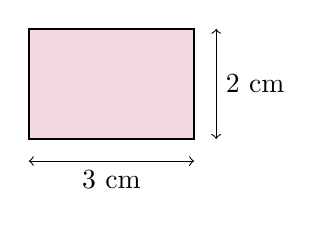
\begin{tikzpicture}[scale=0.7]
  \draw[thick,fill=purple!15] (0,0) rectangle (3,2);
  \draw[<->] (0,-0.4) -- (3,-0.4);
  \node[below] at (1.5,-0.4) {$3$ cm};
  \draw[<->] (3.4,0) -- (3.4,2);
  \node[right] at (3.4,1) {$2$ cm};
\end{tikzpicture}
\end{center}
\end{questionText}
\correctAnswer{$6$ cm by $4$ cm; area $= 24$ cm$^2$}
\explanation{Scale ratio: $\frac{8}{4} = 2$. New dimensions: $3 \times 2 = 6$ cm and $2 \times 2 = 4$ cm. Area: $6 \times 4 = 24$ cm$^2$.}
\end{practiceQuestion}

\begin{practiceQuestion}{6-3-q30}{gsa}
\begin{questionText}
The diagram below shows a triangle attempt with the given side lengths. Explain whether this triangle is possible using the triangle inequality.

\begin{center}
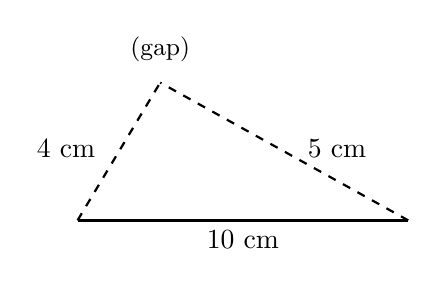
\begin{tikzpicture}[scale=0.7]
  \draw[thick] (0,0) -- (6,0);
  \draw[thick,dashed] (0,0) -- (1.5,2.5);
  \draw[thick,dashed] (6,0) -- (1.5,2.5);
  \node[below] at (3,0) {$10$ cm};
  \node[left] at (0.5,1.3) {$4$ cm};
  \node[right] at (4,1.3) {$5$ cm};
  \node[above] at (1.5,2.7) {\small (gap)};
\end{tikzpicture}
\end{center}
\end{questionText}
\correctAnswer{No, it is not possible}
\explanation{Check: $4 + 5 = 9 < 10$. The two shorter sides cannot connect across the base. The triangle inequality fails, so no triangle can be formed. The dashed lines with the gap illustrate that the sides don't meet.}
\end{practiceQuestion}

\begin{practiceQuestion}{6-4-q24}{sa}
\begin{questionText}
You are given two sides ($5$ cm and $7$ cm) and the included angle ($90°$). Is the resulting triangle unique? What type of triangle is it?
\end{questionText}
\correctAnswer{Yes, unique; it is a right triangle}
\explanation{SAS produces a unique triangle. The included angle of $90°$ makes it a right triangle with legs $5$ cm and $7$ cm.}
\end{practiceQuestion}

\begin{practiceQuestion}{6-5-q19}{sa}
\begin{questionText}
What shape is the cross-section when you cut a sphere through its center?
\end{questionText}
\correctAnswer{A circle (the largest possible circle)}
\explanation{A cut through the center of a sphere produces a great circle — the largest possible circular cross-section, with the same radius as the sphere.}
\end{practiceQuestion}

\begin{practiceQuestion}{6-8-q13}{mc}
\begin{questionText}
Two similar pentagons have a scale factor of $4$. If a side of the smaller pentagon is $3$ cm, what is the corresponding side of the larger pentagon?
\end{questionText}
\choiceA{$7$ cm}
\choiceB{$12$ cm}
\choiceC{$16$ cm}
\choiceD{$0.75$ cm}
\correctAnswer{B}
\explanation{Larger side $= 3 \times 4 = 12$ cm.}
\end{practiceQuestion}

\begin{practiceQuestion}{7-4-q16}{mc}
\begin{questionText}
A figure is made of a right triangle with legs $6$ cm and $8$ cm, and a rectangle $8$ cm by $3$ cm. What is the total area?
\end{questionText}
\choiceA{$24$ cm$^2$}
\choiceB{$48$ cm$^2$}
\choiceC{$36$ cm$^2$}
\choiceD{$72$ cm$^2$}
\correctAnswer{B}
\explanation{Triangle: $\frac{1}{2} \times 6 \times 8 = 24$ cm$^2$. Rectangle: $8 \times 3 = 24$ cm$^2$. Total: $24 + 24 = 48$ cm$^2$.}
\end{practiceQuestion}

\begin{practiceQuestion}{7-5-q09}{mc}
\begin{questionText}
A rectangular prism has dimensions $7$ m by $4$ m by $3$ m. What is the area of the largest face?
\end{questionText}
\choiceA{$12$ m$^2$}
\choiceB{$21$ m$^2$}
\choiceC{$28$ m$^2$}
\choiceD{$84$ m$^2$}
\correctAnswer{C}
\explanation{The three pairs of faces have areas $7 \times 4 = 28$, $7 \times 3 = 21$, and $4 \times 3 = 12$ m$^2$. The largest is $28$ m$^2$.}
\end{practiceQuestion}

\begin{practiceQuestion}{7-6-q12}{mc}
\begin{questionText}
A pool is $10$ m long, $5$ m wide, and $2$ m deep. How many cubic meters of water does it hold when full?
\end{questionText}
\choiceA{$17$ m$^3$}
\choiceB{$50$ m$^3$}
\choiceC{$100$ m$^3$}
\choiceD{$200$ m$^3$}
\correctAnswer{C}
\explanation{$V = 10 \times 5 \times 2 = 100$ m$^3$.}
\end{practiceQuestion}

\begin{practiceQuestion}{8-1-q08}{mc}
\begin{questionText}
A sample of $40$ out of $2{,}000$ voters is surveyed. What fraction of the population is in the sample?
\end{questionText}
\choiceA{$\frac{1}{50}$}
\choiceB{$\frac{1}{40}$}
\choiceC{$\frac{1}{20}$}
\choiceD{$\frac{1}{500}$}
\correctAnswer{A}
\explanation{$\frac{40}{2{,}000} = \frac{1}{50}$.}
\end{practiceQuestion}

\begin{practiceQuestion}{8-2-q26}{gmc}
\begin{questionText}
The dot plot shows the number of books read last month by a random sample of $20$ students.

\begin{center}
\begin{tikzpicture}[scale=0.7]
  \draw[thick,->] (-0.5,0) -- (8.5,0);
  \foreach \x in {0,...,8} {
    \draw (\x,0.1) -- (\x,-0.1);
    \node[below] at (\x,0) {\small $\x$};
  }
  \node[below] at (4,-0.7) {\small Books Read};
  % dots: 0(1), 1(2), 2(4), 3(5), 4(3), 5(3), 6(1), 7(1)
  \fill[funBlue] (0,0.4) circle (0.12);
  \fill[funBlue] (1,0.4) circle (0.12); \fill[funBlue] (1,0.7) circle (0.12);
  \fill[funBlue] (2,0.4) circle (0.12); \fill[funBlue] (2,0.7) circle (0.12);
  \fill[funBlue] (2,1.0) circle (0.12); \fill[funBlue] (2,1.3) circle (0.12);
  \fill[funBlue] (3,0.4) circle (0.12); \fill[funBlue] (3,0.7) circle (0.12);
  \fill[funBlue] (3,1.0) circle (0.12); \fill[funBlue] (3,1.3) circle (0.12);
  \fill[funBlue] (3,1.6) circle (0.12);
  \fill[funBlue] (4,0.4) circle (0.12); \fill[funBlue] (4,0.7) circle (0.12);
  \fill[funBlue] (4,1.0) circle (0.12);
  \fill[funBlue] (5,0.4) circle (0.12); \fill[funBlue] (5,0.7) circle (0.12);
  \fill[funBlue] (5,1.0) circle (0.12);
  \fill[funBlue] (6,0.4) circle (0.12);
  \fill[funBlue] (7,0.4) circle (0.12);
\end{tikzpicture}
\end{center}

What is the mean number of books read in this sample?
\end{questionText}
\choiceA{$2.5$}
\choiceB{$3$}
\choiceC{$3.2$}
\choiceD{$3.5$}
\correctAnswer{C}
\explanation{Sum: $0(1)+1(2)+2(4)+3(5)+4(3)+5(3)+6(1)+7(1) = 0+2+8+15+12+15+6+7 = 65$. Mean: $\frac{65}{20} = 3.25 \approx 3.2$.}
\end{practiceQuestion}

\begin{practiceQuestion}{8-4-q13}{mc}
\begin{questionText}
Store A daily sales: mean $\$500$, MAD $\$40$. Store B daily sales: mean $\$620$, MAD $\$40$. The difference in means in MADs is:
\end{questionText}
\choiceA{$1.5$ MADs}
\choiceB{$3$ MADs}
\choiceC{$40$ MADs}
\choiceD{$120$ MADs}
\correctAnswer{B}
\explanation{Difference $= \$620 - \$500 = \$120$. In MADs: $\frac{120}{40} = 3$ MADs.}
\end{practiceQuestion}

\begin{practiceQuestion}{8-5-q15}{mc}
\begin{questionText}
What is the mean of the data shown?

\begin{center}
\begin{tabular}{r|l}
\textbf{Stem} & \textbf{Leaf} \\
\hline
$1$ & $0\;\;5$ \\
$2$ & $0\;\;5$ \\
$3$ & $0$
\end{tabular}
\end{center}
\end{questionText}
\choiceA{$15$}
\choiceB{$18$}
\choiceC{$20$}
\choiceD{$25$}
\correctAnswer{C}
\explanation{Data: $10, 15, 20, 25, 30$. Mean $= \frac{10+15+20+25+30}{5} = \frac{100}{5} = 20$.}
\end{practiceQuestion}

\begin{practiceQuestion}{8-6-q19}{sa}
\begin{questionText}
A circle graph shows $35\%$ for music, $25\%$ for art, and the rest for drama. What percent is drama?
\end{questionText}
\correctAnswer{$40\%$}
\explanation{$100\% - 35\% - 25\% = 40\%$.}
\end{practiceQuestion}

\begin{practiceQuestion}{9-4-q30}{gsa}
\begin{questionText}
The table below shows a probability model for a game spinner. One probability is missing. Find the missing probability for outcome D.

\begin{center}
\begin{tabular}{|c|c|}
\hline
\textbf{Outcome} & \textbf{Probability} \\
\hline
A & $0.30$ \\
\hline
B & $0.25$ \\
\hline
C & $0.15$ \\
\hline
D & ? \\
\hline
\end{tabular}
\end{center}
\end{questionText}
\correctAnswer{$0.30$}
\explanation{$P(D) = 1 - (0.30 + 0.25 + 0.15) = 1 - 0.70 = 0.30$.}
\end{practiceQuestion}

\begin{practiceQuestion}{9-6-q06}{mc}
\begin{questionText}
Two dice are rolled. What is the probability that both dice show the same number (doubles)?
\end{questionText}
\choiceA{$\frac{1}{36}$}
\choiceB{$\frac{1}{12}$}
\choiceC{$\frac{1}{6}$}
\choiceD{$\frac{1}{3}$}
\correctAnswer{C}
\explanation{Doubles: $(1,1), (2,2), (3,3), (4,4), (5,5), (6,6)$ — that is $6$ out of $36$. $P = \frac{6}{36} = \frac{1}{6}$.}
\end{practiceQuestion}

\begin{practiceQuestion}{9-7-q25}{sa}
\begin{questionText}
A student runs $200$ simulation trials for an event with theoretical probability $\frac{1}{4}$. They observe the event $54$ times. What is the experimental probability? Is it close to the theoretical value?
\end{questionText}
\correctAnswer{$0.27$; yes, it is close to $0.25$}
\explanation{$P = \frac{54}{200} = 0.27$. Theoretical $= 0.25$. The difference of $0.02$ is small, especially with $200$ trials.}
\end{practiceQuestion}
